




与前面类似，张量既能转化为矩阵，也能转化为向量。这一过程称为向量化：
\begin{definition}（向量化）\label{def:vectorization}
设 $\Tt\in\RR^{d_1\times d_2\times\cdots\times d_N}$。$\Tt$ 的\emph{向量化}记为 $\vectorize(\Tt)\in\RR^{d_1d_2\cdots d_N}$，它是把自身的模 $N$ 纤维拼接起来所得到的向量\footnote{按字典序拼接。}。例如，张量 $\Tt\in\RR^{d_1\times d_2\times d_3}$ 的向量化为：
$$\vectorize(\Tt) =    
[(\Tt_{1,1,:})\ \  (\Tt_{1,2,:})\ \  \cdots \ \ (\Tt_{d_1,d_2,:})]^\ts
=
\begin{tikzpicture}[baseline=\baseline]
    \tikzset{tensor/.style = {minimum size = 0.5cm,shape = circle,thick,draw=black,inner sep = 0pt}, edge/.style = {thick,line width=.4mm},every loop/.style={}}
    \def\y{0}
    \def\x{0}
    \node[tensor,fill=blue!10!white] (A) at (\x,\y){\scalebox{0.85}{$\Tt$}};
    \draw[edge] (\x+0.15,\y+0.2) -- (\x+0.5,\y+0.2) -- (\x+0.5,\y+0.1) -- (\x+1,\y+0.1) node [midway,above]
    {\scalebox{0.7}{\dimcolor{$d_1$}}};
     \draw[edge] (A) -- (\x+1,\y)node [right]
    {\scalebox{0.7}{\dimcolor{$d_2$}}};

    \draw[edge] (\x+0.15,\y-0.2) -- (\x+0.5,\y-0.2)-- (\x+0.5,\y-0.1)-- (\x+1,\y-0.1) node [midway,below]
    {\scalebox{0.7}{\dimcolor{$d_3$}}};
    \end{tikzpicture}\in\RR^{d_1d_2d_3}.
$$
\end{definition}

向量化是一种展开操作，它把任意阶的张量化为向量。与矩阵化类似，在张量网络中，形如
$
\begin{tikzpicture}[baseline=\baseline]
    \tikzset{tensor/.style = {minimum size = 0.5cm,shape = circle,thick,draw=black,inner sep = 0pt}, edge/.style = {thick,line width=.4mm},every loop/.style={}}
    \def\y{0}
    \def\x{0}
    \draw[edge] (\x+0.15,\y+0.2) -- (\x+0.5,\y+0.2) -- (\x+0.5,\y+0.1) -- (\x+1,\y+0.1) node [midway,above]
    {\scalebox{0.7}{\textcolor{gray}{$d_1$}}};
    \draw[edge] (\x+0.15,\y) -- (\x+1,\y)node [right]
    {\scalebox{0.7}{\textcolor{gray}{$d_2$}}};
    \draw[edge] (\x+0.15,\y-0.2) -- (\x+0.5,\y-0.2)-- (\x+0.5,\y-0.1)-- (\x+1,\y-0.1) 
node [midway,below]
    {\scalebox{0.7}{\dimcolor{$d_3$}}};
    \end{tikzpicture}
$ 的边表示一条大小为 $d_1d_2d_3$ 的边。一般而言，全文中汇聚于一点的边表示一条边，其大小等于所有相关边大小之积。注意，张量的向量化等于该张量模 $1$ 矩阵化的向量化\footnote{为与本书所用的向量化定义保持一致，矩阵的向量化由其各行拼接而成，这有时称为\emph{行主序向量化}。注意，这正是 \textsf{Python} 中 \textsf{numpy} 包默认的向量化操作 \textsf{ravel()}。}，即对 $\Tt\in\RR^{d_1\times d_2\cdots \times d_N}$，有 $\vectorize(\Tt) = \vectorize(\Tt_{(1)})$。




\subsection{乘积}\label{sec:product}
张量可以用不同类型的运算组合起来，即进行各种\textit{乘法}。本节给出各类乘积运算的图示。
\paragraph{模 $n$ 张量乘积}\label{par:mode-n-tensor-product}
模 $n$ 乘积是张量沿某个特定的模与矩阵相乘，可视为矩阵乘法的推广。更确切地说，模 $n$ 乘积把矩阵与矩阵的乘法推广到某一个特定的模上，其中包括张量与矩阵、以及张量与向量之间的模 $n$ 乘积。
\begin{enumerate}
\item \textbf{模-n 乘积~（矩阵）。}\label{subsec:mode-n}
    张量 $\Xt\in\RR^{d_1\times\cdots\times d_N}$ 与矩阵 $\Mb\in\RR^{m\times d_n}$ 的模 $n$ 乘积记为
    $\Xt\ttm n \Mb \in \RR^{d_1\times \cdots\times d_{n-1}\times m\times d_{n+1}\times\cdots\times d_N}$，其定义为张量与矩阵沿张量的模 $n$、沿矩阵的第二模~（列指标）收缩，即 
    $$
  \Xt\ttm n \Mb
=
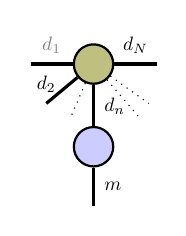
\begin{tikzpicture}[baseline=-0.5ex]
    \tikzset{tensor/.style = {minimum size = 0.5cm,shape = circle,thick,draw=black,inner sep = 0pt}, edge/.style = {thick,line width=.4mm},every loop/.style={}}
    \def\x{6}
    \node[tensor,fill=blue!20!white] (M) at (\x,-1.05) {$\Mb$};
    \node[tensor,fill=green!50!red!50!white] (At) at (\x,0) {$\Xt$};
    \draw[edge] (At) -- (\x-0.8,0) node [midway,above] {\scalebox{0.7}{\textcolor{gray}{$d_1$}}};
    \draw[edge] (At)-- (\x-0.6,-0.5) node [above]{\scalebox{0.7}{\dimcolor{$d_2$}}};
    \draw[edge] (At) -- (\x+0.8,0) node [midway,above] {\scalebox{0.7}{\dimcolor{$d_N$}}};;
    \draw[dotted] (At) -- (\x-0.3,-0.7);
    \draw[edge] (At) -- (\x,-0.8) node [midway,right] {\scalebox{0.7}{\dimcolor{$d_n$}}};
    \draw[dotted] (At) -- (\x+0.6,-0.7);
    \draw[dotted] (At) -- (\x+0.7,-0.5);
    \draw[edge] (M) -- (\x,-1.8) node [midway,right] {\scalebox{0.7}{\dimcolor{$m$}}};;
    \end{tikzpicture}
\in\RR^{d_1\times  \dots\times d_{n-1}\times m \times d_{n+1}\times \dots\times d_N}.
$$
该运算把张量的第 $n$ 模与矩阵的第二模~（列）收缩，原来的维数 $d_n$ 被新维数 $m$ 取代。若 $\Ab\in\RR^{d_n\times n},\Bb\in\RR^{d_m\times m}$ 与 $\Xt\in\RR^{d_1\times\cdots\times d_N}$ 所对应的模 $n\neq m$ 互不相同，则相乘的顺序无关紧要，即
$$
\Xt\ttm n \Ab \ttm m \Bb = 
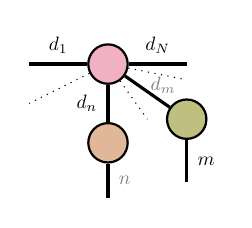
\begin{tikzpicture}[baseline=-0.5ex]
    \tikzset{tensor/.style = {minimum size = 0.5cm,shape = circle,thick,draw=black,inner sep = 0pt}, edge/.style = {thick,line width=.4mm},every loop/.style={}}
    \def\x{0}
    \def\y{0}
    \node[tensor,fill=blue!20!red!30!white] (Xt) at (\x,\y) {$\Xt$};
    \node[tensor,fill=green!30!red!40!white] (A) at (\x,\y-1) {$\Ab$};
    \node[tensor,fill=green!50!red!50!white] (B) at (\x+1,\y-0.7) {$\Bb$};
    \draw[edge] (Xt) -- (\x-1,\y) node [midway,above] {\scalebox{0.7}{\dimcolor{$d_1$}}};
    \draw[dotted] (Xt) -- (\x-1,\y-0.5);
    \draw[edge] (Xt) -- (\x+1,\y) node [midway,above] {\scalebox{0.7}{\dimcolor{$d_N$}}};
    \node[draw=none] () at (\x+0.7,\y-0.27) {\scalebox{0.7}{\textcolor{gray}{$d_m$}}};
    \draw[edge] (Xt) -- (A) node [midway,left] {\scalebox{0.7}{\dimcolor{$d_n$}}};
    \draw[edge] (A) -- (\x,\y-1.7) node [midway,right] {\scalebox{0.7}{\textcolor{gray}{$n$}}};
    \draw[edge] (Xt) -- (B);
    \draw[edge] (B) -- (\x+1,\y-1.5) node [midway,right] {\scalebox{0.7}{\dimcolor{$m$}}};
    \draw[dotted] (Xt) -- (\x+1,\y-0.2);
    \draw[dotted] (Xt) -- (\x+0.5,\y-0.7);
    \end{tikzpicture}
= \Xt\ttm m\Bb\ttm n \Ab,~~\text{For}~~n\neq m.
$$
然而当 $m = n$ 时，乘积的顺序就至关重要。特别地，若 $\Ab\in\RR^{n\times d_n}$、$\Bb\in\RR^{p\times n}$，则 $(\Xt\ttm n \Ab) \ttm n \Bb = \Xt\ttm n(\Bb\Ab)$，而乘积 $(\Xt\ttm n \Bb) \ttm n \Ab$ 仅当 $n=d_n=p$ 时才有意义。
模 $n$ 张量乘积可以视为经典矩阵乘法的推广。特别地，
用二阶张量的模 $1$ 乘积与模 $2$ 乘积即可还原出矩阵乘积：
若 $\Ab\in\RR^{m\times n}$、$\Bb\in\RR^{p\times n}$、$\Cb\in\RR^{d\times m}$，则
\begin{align*}
\Ab\ttm2 \Bb
=
\begin{tikzpicture}[baseline=\baseline]
   \tikzset{tensor/.style = {minimum size = 0.5cm,shape = circle,thick,draw=black,inner sep = 0pt}, edge/.style = {thick,line width=.4mm},every loop/.style={}}
    \def\y{0}
    \def\x{0}
    \node[tensor,fill=red!50!white] (A) at (\x,\y){\scalebox{0.85}{$\Ab$}};
    \node[tensor,fill=blue!50!white] (B) at (\x+1,\y){\scalebox{0.85}{$\Bb$}};
    \draw[edge] (A) -- (B) node [above,midway] {\scalebox{0.7}{\dimcolor{$n$}}};
    \draw[edge] (\x-0.25,\y) -- (\x-0.6,\y)  node [midway,above] {\scalebox{0.7}{\dimcolor{$m$}}};
    \draw[edge] (\x+1.25,\y) -- (\x+1.6,\y)  node [midway,above] {\scalebox{0.7}{\dimcolor{$p$}}};
    \end{tikzpicture}
    = \Ab\Bb^\ts\in\RR^{m\times p},
\end{align*}
\begin{align*}
    \Ab\ttm1 \Cb =
    \begin{tikzpicture}[baseline=\baseline]
   \tikzset{tensor/.style = {minimum size = 0.5cm,shape = circle,thick,draw=black,inner sep = 0pt}, edge/.style = {thick,line width=.4mm},every loop/.style={}}
    \def\y{0}
    \def\x{0}
    \node[tensor,fill=red!20!white] (C) at (\x,\y){\scalebox{0.85}{$\Cb$}};
    \node[tensor,fill=red!50!white] (A) at (\x+1,\y){\scalebox{0.85}{$\Ab$}};
    \draw[edge] (C) -- (A) node [above,midway] {\scalebox{0.7}{\dimcolor{$m$}}};
    \draw[edge] (\x-0.25,\y) -- (\x-0.6,\y)  node [midway,above] {\scalebox{0.7}{\dimcolor{$d$}}};
    \draw[edge] (\x+1.25,\y) -- (\x+1.6,\y)  node [midway,above] {\scalebox{0.7}{\dimcolor{$n$}}};
    \end{tikzpicture}
    = \Cb\Ab\in\RR^{d\times n}.
\end{align*}

